% =============================================================================
% INITIAL DRAFT -- Paper A (Mathematical Methods in the Applied Sciences)
%
% Generated as part of the two-paper research plan in ../PLAN.md. Uses a
% portable `article` preamble (matching docs/CALL_FOR_PAPERS.tex) as a stand-in
% for the official Wiley WileyNJD-v2 class, which should be substituted before
% submission (see PLAN.md sec. 8). All numeric results are MOCK PLACEHOLDERS --
% see the draft-status banner below and PLAN.md sec. 5 for the labeling
% convention. Figures under "Results" are `\figureplaceholder{}` boxes with no
% external image dependency; methodology/dataset figures reuse real existing
% assets from docs/plots/.
% =============================================================================
\documentclass[11pt,a4paper]{article}

\usepackage[utf8]{inputenc}
\usepackage[T1]{fontenc}
\usepackage{geometry}
\geometry{top=1in, bottom=1in, left=1in, right=1in}
\usepackage{amsmath}
\usepackage{amssymb}
\usepackage{microtype}
\usepackage{graphicx}
\usepackage{booktabs}
\usepackage{multirow}
\usepackage{xcolor}
\usepackage{cite}
\usepackage{hyperref}

\graphicspath{{../../docs/plots/}}

\hypersetup{
    colorlinks=true,
    linkcolor=blue,
    filecolor=magenta,
    urlcolor=cyan,
    citecolor=blue,
}

% ---- Mock-data / placeholder conventions (see PLAN.md sec. 5) ----------------
\newcommand{\mocknote}{{\footnotesize\color{red!60!black}\textit{(Mock data --- placeholder pending real experiments; see Section~\ref{sec:reproducibility}.)}}}
\newcommand{\figureplaceholder}[2]{%
\begin{figure}[ht]
\centering
\setlength{\fboxsep}{0pt}
\fbox{\begin{minipage}[c][0.28\textheight][c]{0.85\textwidth}
\centering
{\color{gray}\rule{0.8\textwidth}{0.4pt}}\\[0.8em]
{\bfseries\color{gray!60!black} FIGURE PLACEHOLDER}\\[0.4em]
{\color{gray!70!black}\itshape pending real experiment}\\[0.8em]
{\color{gray}\rule{0.8\textwidth}{0.4pt}}
\end{minipage}}
\caption{#2}
\label{fig:#1}
\end{figure}}

\title{\textbf{Physics-Informed Contrastive Representation Learning for Self-Supervised Anomaly Detection in Power Converter Frequency-Response Signatures}}

\author{
    \textbf{Ignacio Martin-Salinas}, \textbf{Jose A. Belloch}, \textbf{Cristina Fernandez} \\
    \small Depto. de Tecnolog\'{i}a Electr\'{o}nica, Universidad Carlos III de Madrid, Madrid, Spain
}
\date{}

\begin{document}
\maketitle

\begin{center}
\fcolorbox{red!60!black}{red!5}{\begin{minipage}{0.92\textwidth}
\small\textbf{Draft status.} This is an \emph{initial draft} generated to scaffold the
manuscript structure and methodology description. All quantitative results (tables and
figures under Section~\ref{sec:results}) are \textbf{mock placeholders} pending the
completion of a CARLA retrain under the current physics-informed anomaly injector (see
Section~\ref{sec:reproducibility}). Do not cite or circulate the numeric results in this
draft as findings.
\end{minipage}}
\end{center}

\begin{abstract}
Faults in power electronic converters precede catastrophic failure with subtle,
non-linear parametric drift that simple threshold alarms cannot resolve. This paper
studies self-supervised anomaly detection directly on the converter's frequency-domain
transfer-function (Bode) signature, extending the CARLA (Contrastive Representation
Learning for Anomaly Detection) framework with a \emph{physics-informed negative
sampler}: rather than perturbing the signal with generic heuristics, candidate negative
samples are synthesized by perturbing the converter's own small-signal component values
and analytically re-deriving the resulting transfer function, yielding hard negatives
that are physically consistent with the converter under test. We formalize the
labeling problem as a set-membership rule over component-wise multiplier bands
grounded in manufacturing-tolerance and degradation standards, describe a Latin
Hypercube sampling strategy for both the healthy and multi-fault regimes, and compare
the physics-informed contrastive encoder against six autoencoder baselines (Conv1D,
LSTM, GRU, MLP, VAE, Transformer) and against a heuristic-negative-sampling ablation of
CARLA itself. On the held-out test set, the physics-informed CARLA variant achieves an
F1-score of \textbf{[MOCK]} and ROC-AUC of \textbf{[MOCK]}, compared with
\textbf{[MOCK]} / \textbf{[MOCK]} for the heuristic-negative ablation and
\textbf{[MOCK]} / \textbf{[MOCK]} for the strongest reconstruction-only baseline
(placeholders pending retraining; see Section~\ref{sec:reproducibility}). We discuss the
implications of physically grounded negative synthesis for representation collapse and
sample efficiency in contrastive time-series anomaly detection.
\end{abstract}

\noindent\textbf{Keywords:} Anomaly Detection; Power Electronics; Self-Supervised Learning;
Contrastive Representation Learning; Autoencoders; Transfer Function; Physics-Informed
Machine Learning

\section{Introduction}
\label{sec:intro}

Power electronic converters are foundational components of aerospace platforms, electric
vehicles, and increasingly renewable-dominated power grids~\cite{idrisov2025digitaltwin}.
Component-level degradation --- capacitor dielectric wear-out, inductor core saturation,
MOSFET on-resistance drift --- develops gradually and non-linearly, and precedes outright
failure by a substantial margin. Traditional condition monitoring relies on manual
inspection or fixed-threshold alarms on a handful of scalar indicators, both of which are
insensitive to the joint, multi-component nature of real degradation and to failure modes
that were not anticipated at commissioning time~\cite{liu2022review,kou2022faultdiagnosis}.

Data-driven anomaly detection offers an alternative: rather than hand-designing fault
signatures, a model learns the manifold of \emph{healthy} operating signatures and flags
deviations from it. Recent work has applied this idea to power electronics using
autoencoders, contrastive objectives, and edge-deployable pipelines built on synthetic or
digital-twin data~\cite{beattie2022robust,gomez2023selfcommissioning,idrisov2025digitaltwin}.
Two obstacles recur throughout this literature. First, \textbf{label scarcity}: real fault
data is expensive or unsafe to collect, so most pipelines (including ours) train
exclusively on simulated healthy/faulty transfer functions from a physics-based digital
twin. Second, and more subtle, \textbf{representation collapse} in contrastive setups: if
negative samples are drawn from the training distribution itself (which is overwhelmingly
healthy), the encoder can trivially satisfy the contrastive objective without learning a
discriminative representation~\cite{chen2023harnessing}. CARLA~\cite{darban2023carla}
addresses this by \emph{synthesizing} negative samples rather than mining them, but its
original negative-synthesis operators (spectral noise, time warping, generic amplitude
scaling) are domain-agnostic heuristics with no guarantee of resembling the failure modes
that actually occur in the target system.

This paper's central methodological contribution is to replace those heuristic negative
operators with a \textbf{physics-informed negative sampler}: each synthetic anomaly is
generated by perturbing the converter's own small-signal component values within a
standards-grounded degradation band and \emph{analytically re-deriving} the resulting
transfer function, so that every negative example is a physically realizable converter
state rather than an arbitrary signal distortion. Concretely, we make the following
contributions:
\begin{enumerate}
    \item A formalization of the healthy/anomalous labeling problem for power-converter
    frequency-response signatures as a set-membership rule over standards-grounded,
    component-specific multiplier bands (Section~\ref{sec:problem}), replacing an earlier,
    coarser flat-percentage labeling convention used in preliminary versions of this work.
    \item A Latin Hypercube sampling strategy for both the healthy tolerance box and a
    multi-fault regime (primary fault plus independently-triggered secondary faults),
    implemented as a resumable, manifest-logged data-generation pipeline
    (Section~\ref{sec:dataset}).
    \item A physics-informed negative sampler for CARLA-style contrastive anomaly
    detection (Section~\ref{sec:carla}) and a controlled ablation against the original
    heuristic negative operators (Section~\ref{sec:setup}).
    \item An empirical comparison against six autoencoder architectures under an
    identical hyperparameter-search protocol (Sections~\ref{sec:baselines}
    and~\ref{sec:results}).
\end{enumerate}
A companion manuscript, submitted to the \emph{Journal of Supercomputing}, addresses the
computational optimization and edge-hardware deployment of this framework in depth; this
paper is scoped to the anomaly-detection methodology and its evaluation.

\section{Related Work}
\label{sec:related}

\subsection{Autoencoder-based time-series anomaly detection}
Reconstruction-based anomaly detection trains a model --- typically an autoencoder --- to
reproduce healthy data and scores test samples by reconstruction error. Architectures
range from the original feed-forward formulation~\cite{rumelhart1986backprop} to recurrent
encoders built on LSTM~\cite{hochreiter1997lstm} and GRU~\cite{cho2014gru} cells for
sequential drift, one-dimensional convolutional encoders that exploit local frequency
structure~\cite{kiranyaz2019survey}, attention-based Transformer
encoders~\cite{vaswani2017attention} for long-range dependencies across a frequency sweep,
and probabilistic Variational Autoencoders~\cite{kingma2013autoencoding} that regularize
the latent space via a KL divergence term. Purely reconstruction-based scoring, however,
only penalizes deviation from the healthy manifold and does not explicitly shape a
discriminative decision boundary, motivating hybrid and ensemble
approaches~\cite{zimmerer2018contextvae,gao2020robusttad,campos2021unsupervised} and
renewed attention to evaluation methodology and threshold
selection~\cite{yuan2022trustworthy}.

\subsection{Contrastive and self-supervised learning}
Contrastive learning trains an encoder to pull together representations of related views
of the data while pushing apart unrelated ones, most famously via the NT-Xent objective in
SimCLR~\cite{chen2020simclr}. Applying this idea to time-series anomaly detection is
complicated by the absence of natural negative examples (real faults are rare or absent
at training time); CARLA~\cite{darban2023carla} sidesteps this by \emph{synthesizing}
negatives through heuristic signal perturbations, and further stabilizes training against
representation collapse relative to naive negative
mining~\cite{chen2023harnessing,zhang2025encodethendecompose}. This paper's
physics-informed negative sampler (Section~\ref{sec:carla}) is, to our knowledge, the
first to replace CARLA's domain-agnostic negative operators with an analytic,
component-level perturbation model specific to the monitored system.

\subsection{Data-driven fault diagnosis in power electronics}
Deep learning has been applied to power-converter fault diagnosis via deep feedforward
classifiers on wavelet-compressed features~\cite{kou2022faultdiagnosis}, explainable
anomaly-detection pipelines~\cite{beattie2022robust}, digital-twin-driven anomaly
detection for power-electronics-dominated grids~\cite{idrisov2025digitaltwin}, and
edge-computing-oriented self-commissioning detectors~\cite{gomez2023selfcommissioning}. A
recent survey catalogs AI-based open-circuit fault diagnosis
methods~\cite{liu2022review}. This paper differs from that body of work primarily in its
use of a fully physics-grounded, standards-referenced degradation model both for dataset
labeling (Section~\ref{sec:problem}) and for contrastive negative synthesis
(Section~\ref{sec:carla}), rather than treating faults as either purely data-driven labels
or generic signal perturbations.

\section{Problem Formulation}
\label{sec:problem}

\begin{figure}[ht]
\centering
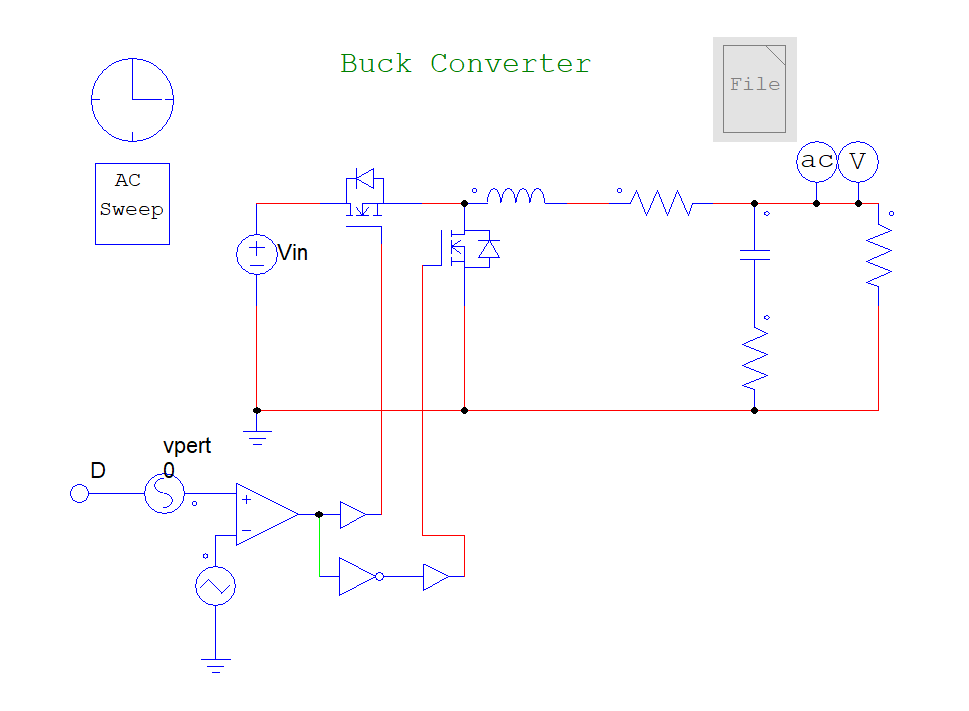
\includegraphics[width=0.62\textwidth]{buck_converter_schematic.png}
\caption{Buck converter topology used as the reference system. Nominal values:
$V_{in}=50\text{ V}$, $L=0.2\text{ mH}$, $C_{out}=100\ \mu\text{F}$, $R_{ds}=10\ \text{m}\Omega$.}
\label{fig:buck-schematic}
\end{figure}

We study a synchronous buck converter (Figure~\ref{fig:buck-schematic}) whose health is
characterized by its small-signal control-to-output transfer function
\begin{equation}
H(s) \;=\; \frac{V_{out}(s)}{V_{in}(s)}\,,
\end{equation}
which for a voltage-mode buck converter with output capacitor ESR $R_{ESR,C}$ takes the
canonical form~\cite{erickson2001fundamentals}
\begin{equation}
G_{vd}(s) \;=\; V_{in}\cdot\frac{1+sR_{ESR,C}C_{out}}{1+s\left(\dfrac{L}{R_{out}}+R_{ESR,C}C_{out}\right)+s^2LC_{out}}\,,
\label{eq:gvd}
\end{equation}
with corner frequencies
\begin{equation}
\omega_0=\frac{1}{\sqrt{LC_{out}}}\,,\qquad
Q=R_{out}\sqrt{\frac{C_{out}}{L}}\,,\qquad
\omega_z=\frac{1}{R_{ESR,C}\,C_{out}}\,.
\label{eq:corner-freqs}
\end{equation}
At the nominal component values in Figure~\ref{fig:buck-schematic}, Eq.~\eqref{eq:corner-freqs}
places the resonant frequency at $f_0=\omega_0/2\pi\approx 1.13\text{ kHz}$, well inside the
$100\text{ Hz}$--$50\text{ kHz}$ measurement band described below, whereas the ESR zero
$\omega_z$ typically falls close to or beyond the upper edge of that band for the healthy
range of $R_{ESR,C}$ --- a fact that, as discussed in Section~\ref{sec:dataset}, makes
inductance and capacitance drift partially degenerate in-band.

\subsection{Degradation as a component-multiplier perturbation}
Let $\boldsymbol\theta=(C_{out}, L, R_{ds,1}, R_{ds,2}, R_{ESR,C}, R_{ESR,L})$ collect the
six components subject to variation, with nominal values $\boldsymbol\theta^{(0)}$. We
define the multiplier vector $\mathbf{m}=\boldsymbol\theta \oslash \boldsymbol\theta^{(0)}$
(element-wise division), so $\mathbf{m}=\mathbf 1$ at nominal. Each component $i$ is
assigned a \emph{normal} band $\mathcal M_i^n$ and an \emph{anomalous} band $\mathcal
M_i^a$ (possibly $\varnothing$ for a pure operating-point knob rather than a fault
mode), grounded in manufacturing-tolerance and degradation
standards~\cite{iec60384_1,waugh_dcbias,kulkarni2010electrolytic,celaya2011mosfet}. For
example, the output-capacitor bands used in the current data-generation pipeline are
$\mathcal M_{C_{out}}^n=[0.80,1.20]$ (manufacturing tolerance) and $\mathcal
M_{C_{out}}^a=[0.30,0.70]$ (capacitance drop $>30\%$, the IEC~60384-4-1 wear-out
criterion), and its ESR bands are $\mathcal M_{ESR,C}^n=[0.50,2.00]$ and $\mathcal
M_{ESR,C}^a=[3.00,8.00]$ (ESR rise $\ge 3\times$ nominal). Analogous, physically grounded
bands for the remaining components are declared in the converter's
\texttt{component\_ranges.json} configuration rather than hard-coded, so that a new
converter topology requires only a new data folder and no code changes.

\subsection{Labeling rule}
A simulated sample is labeled
\begin{equation}
y(\mathbf m)=
\begin{cases}
\textsf{anomalous} & \text{if } \exists\, i:\ m_i\in\mathcal M_i^a,\\
\textsf{normal} & \text{if } \forall i:\ m_i\in\mathcal M_i^n,\\
\textsf{unknown} & \text{otherwise (excluded from training and evaluation).}
\end{cases}
\label{eq:label-rule}
\end{equation}
Each simulated converter state is observed only through its frequency-response signature:
amplitude (dB) and phase (degrees) at $101$ logarithmically spaced frequencies between
$100\text{ Hz}$ and $50\text{ kHz}$, giving a feature vector $x\in\mathbb R^{202}$.

\section{Dataset Generation}
\label{sec:dataset}

Training and evaluation data are produced by a PSIM-based digital twin of the converter in
Figure~\ref{fig:buck-schematic}, avoiding the cost and safety concerns of destructive
physical testing. Two sampling regimes populate the dataset:
\begin{itemize}
    \item \textbf{Healthy set.} Latin Hypercube Sampling (LHS) over the joint tolerance
    box $\prod_i \mathcal M_i^n$, giving stratified, gap-free coverage of the healthy
    operating envelope rather than a fixed percentage grid.
    \item \textbf{Faulty set.} Each sample receives one guaranteed \emph{primary} fault
    (evenly split across the fault-capable components) drawn from that component's
    anomalous band, while every \emph{other} fault-capable component independently
    fails with probability $p_{\text{fault}}$ (default $0.1$), producing a realistic
    mixture of single- and multi-component fault severities rather than assuming faults
    are always isolated. Non-faulted components are drawn from their normal band (not
    held at exact nominal), and all draws are LHS-stratified within their respective
    bands.
\end{itemize}
Every simulation is written under an opaque identifier and its ground-truth multiplier
vector and label are appended in real time to a CSV manifest, making data generation
resumable (grid combinations already present are skipped; LHS runs are topped up to the
requested count) and the labeling fully auditable (Eq.~\eqref{eq:label-rule} applied
directly to the manifest, not re-derived from filenames).

This range-based, standards-grounded, LHS-sampled scheme \textbf{supersedes} an earlier
flat-percentage convention (fixed $\pm5\%$ ``normal'' / $\pm20\%$ ``anomalous'' bands
applied uniformly to all components) used in preliminary internal drafts of this project;
all dataset statistics reported below reflect the current scheme. The final dataset
comprises $N_{\text{total}}=\textbf{[MOCK]}$ labeled signatures \mocknote{}, split
$70\%/15\%/15\%$ into stratified train/validation/test sets.

\begin{figure}[ht]
\centering
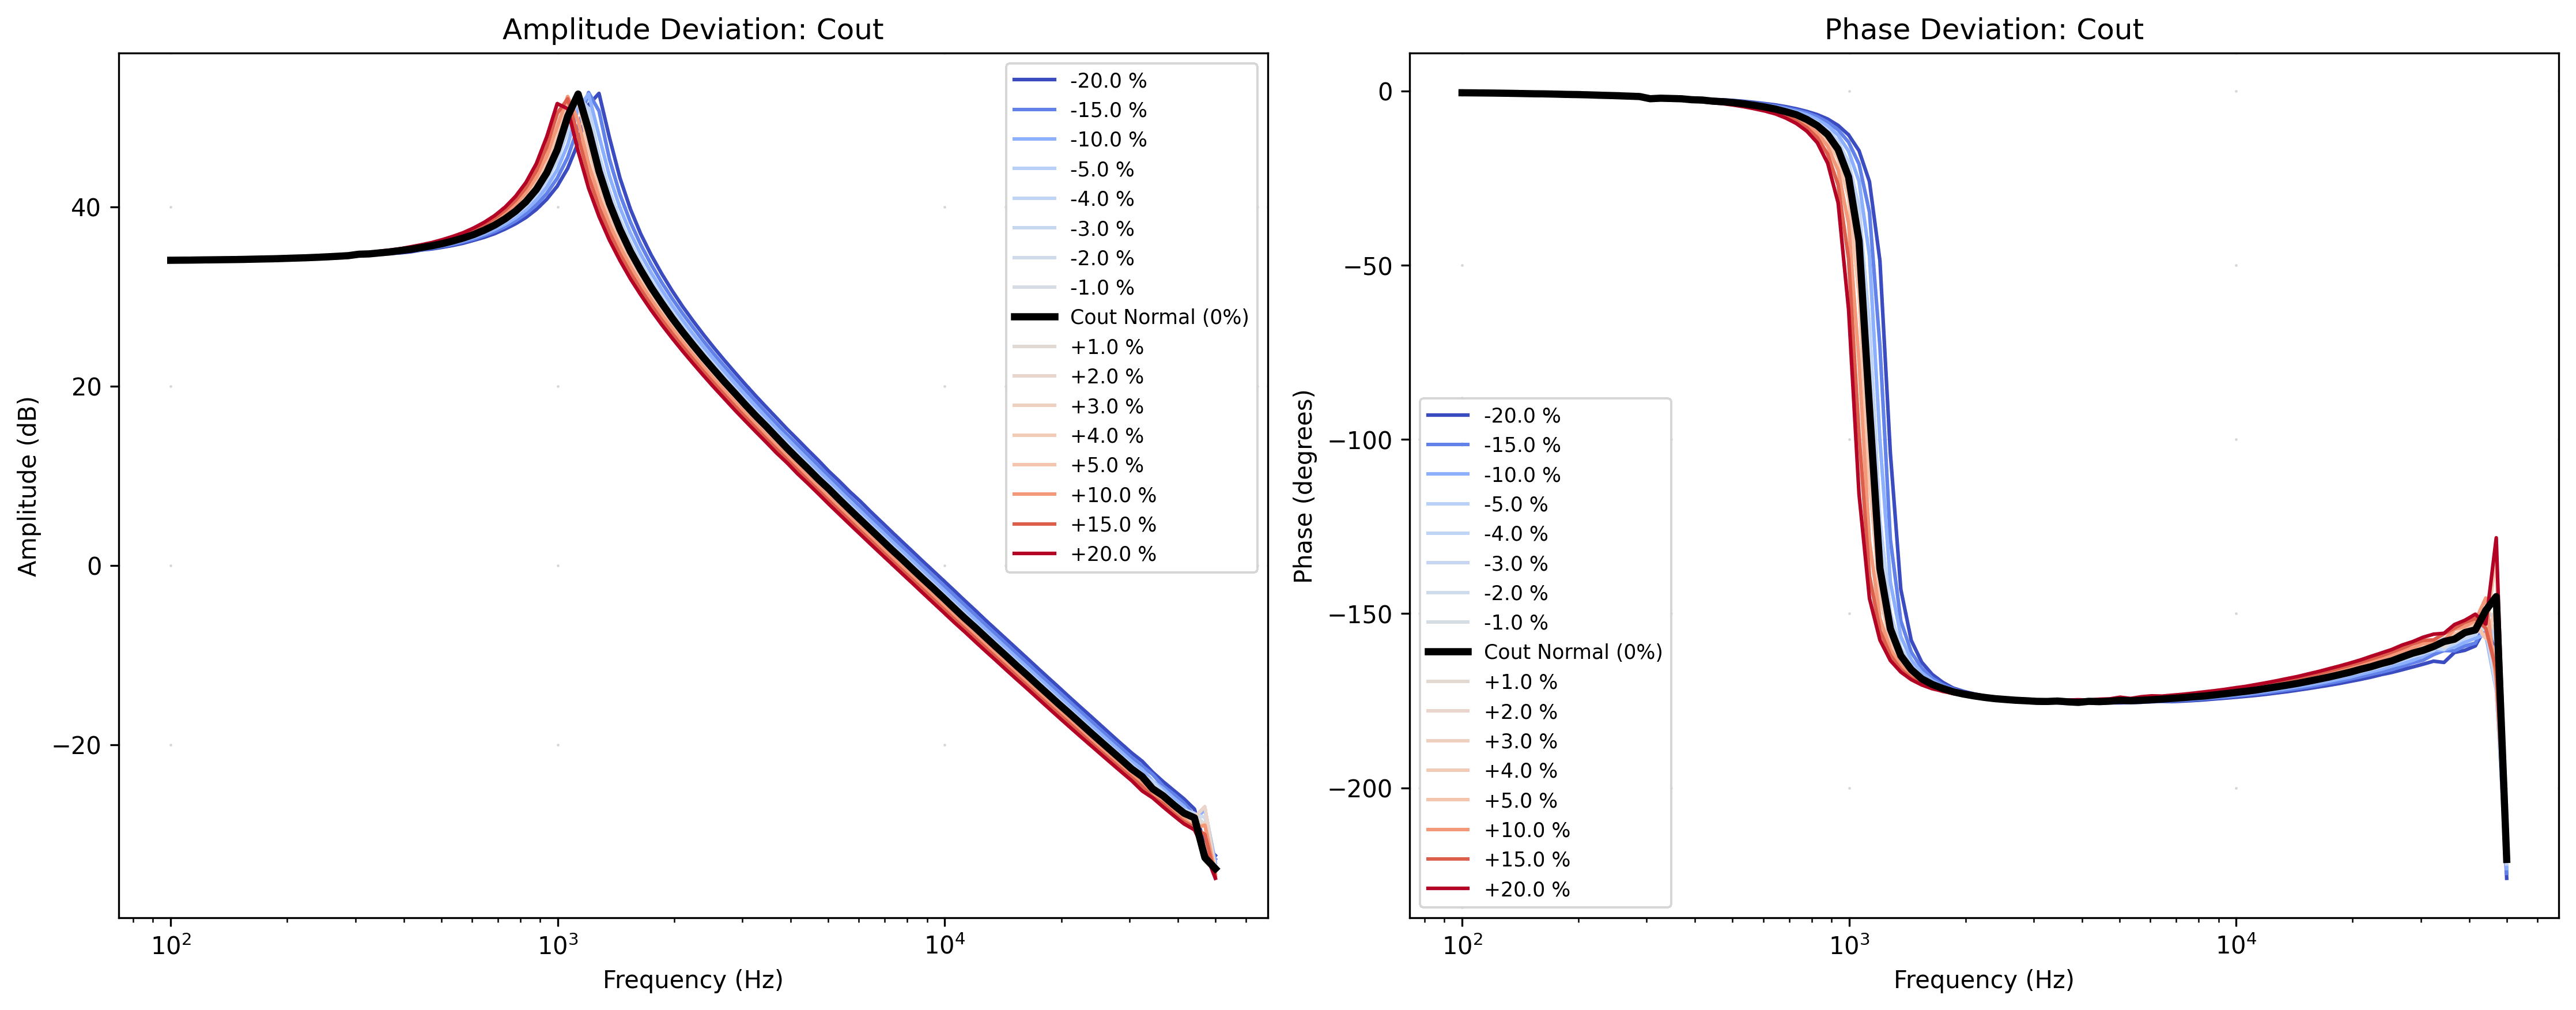
\includegraphics[width=0.48\textwidth]{anomaly_deviation_Cout.png}\hfill
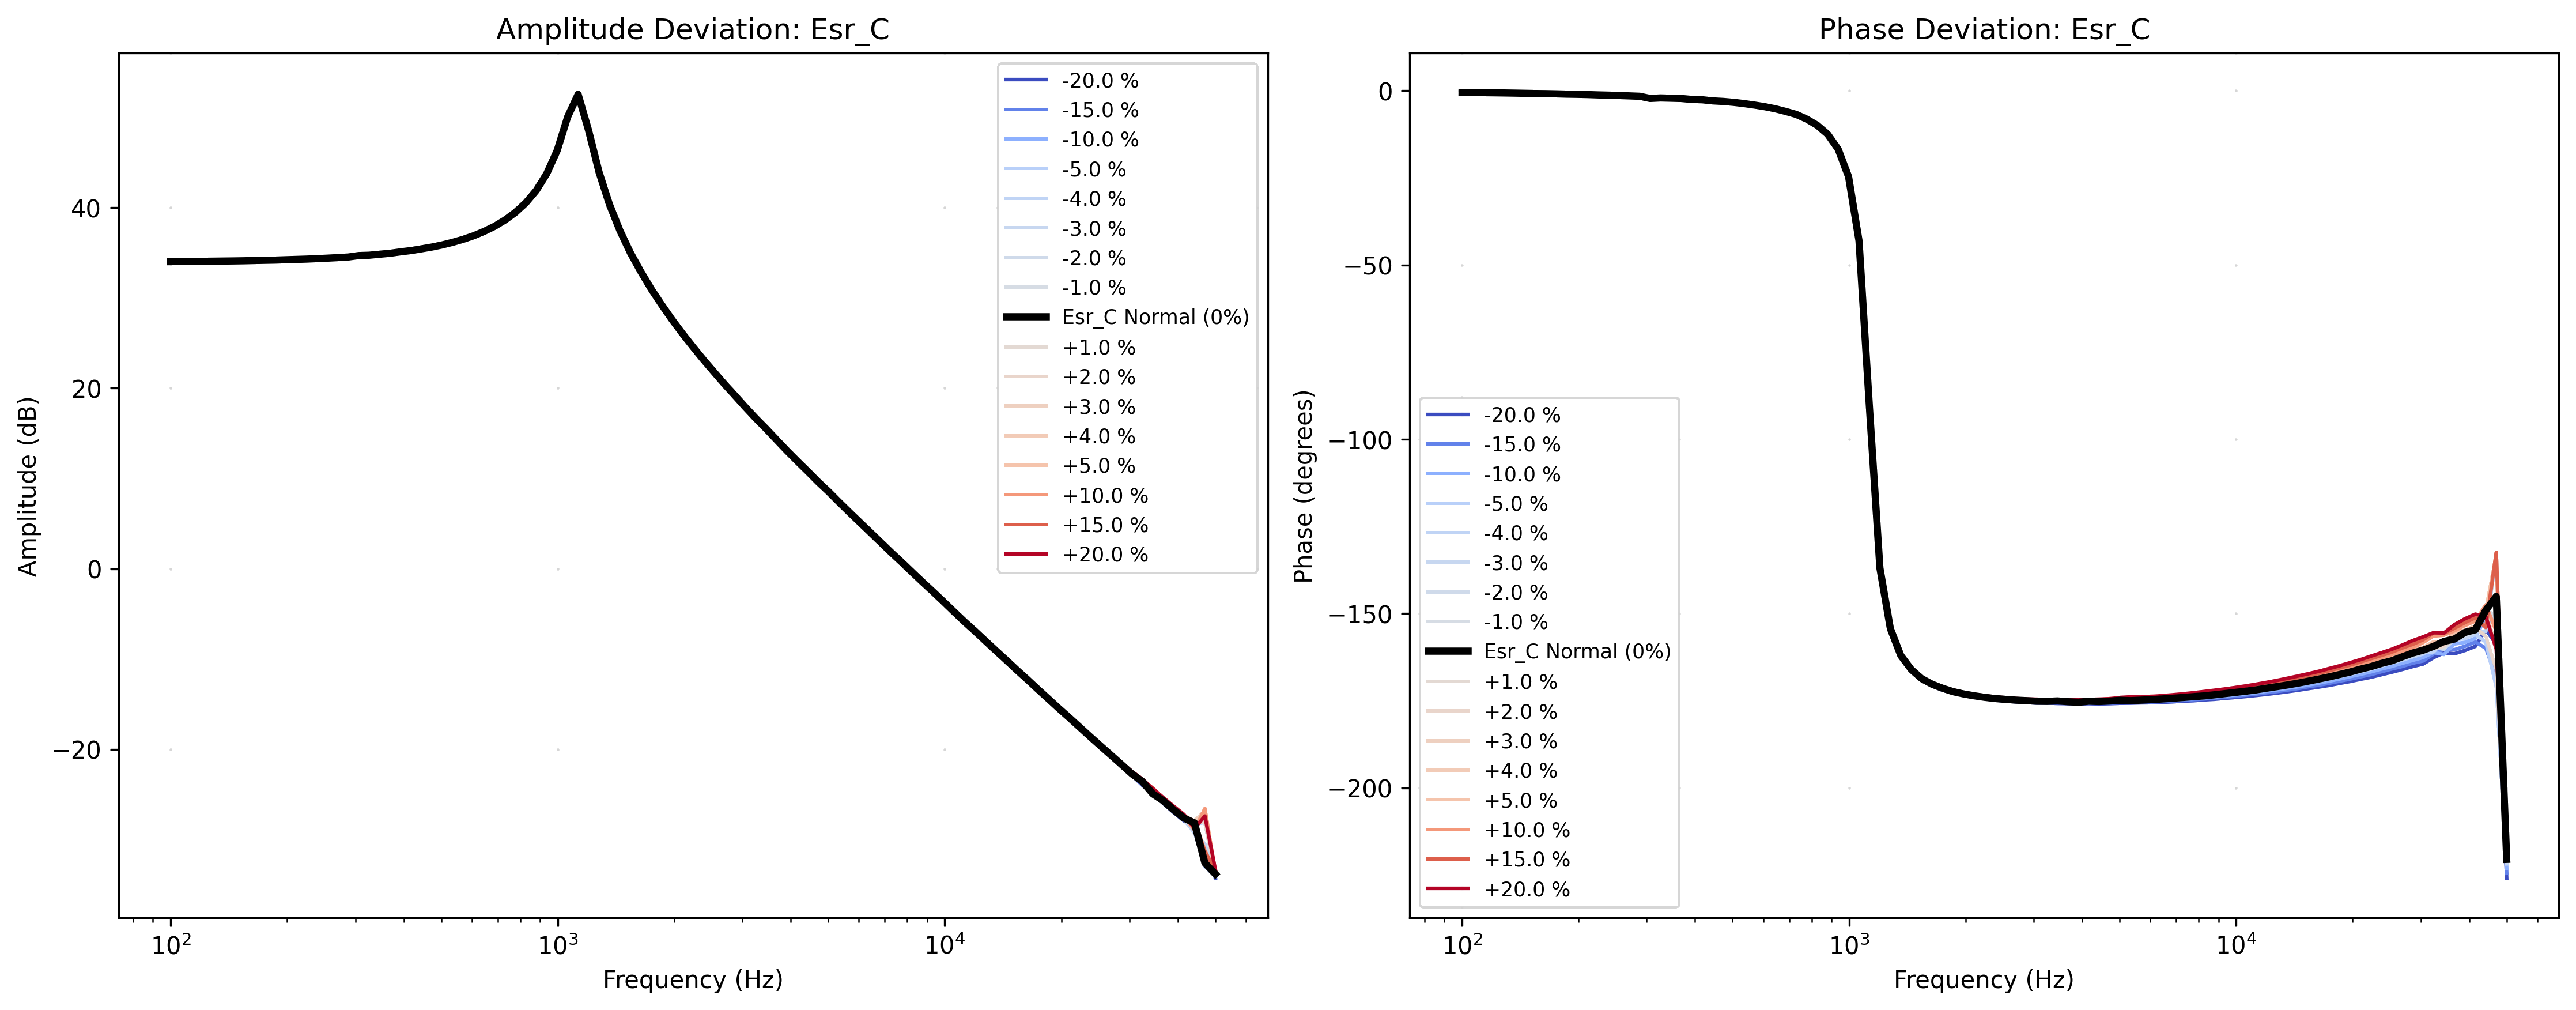
\includegraphics[width=0.48\textwidth]{anomaly_deviation_Esr_C.png}
\caption{Illustrative frequency-response drift under output-capacitance degradation
(left, strong resonance-frequency shift) and capacitor-ESR degradation (right, subtler
high-frequency effect), consistent with the corner-frequency relations in
Eq.~\eqref{eq:corner-freqs}.}
\label{fig:anomaly-deviation-examples}
\end{figure}

\section{Autoencoder Baseline Architectures}
\label{sec:baselines}

All baselines share a common \texttt{BaseAutoencoder} interface (fit/score/save/load) so
that architecture choice is orthogonal to the training and evaluation pipeline. Table
\ref{tab:architectures} summarizes the six baseline architectures and their
architecture-specific hyperparameters; all architectures additionally share a searchable
latent dimension $\in\{16,32,64,128\}$, dropout rate, optional batch normalization, and
activation function $\in\{\text{relu, gelu, swish, mish, elu, leaky\_relu, selu}\}$.

\begin{table}[ht]
\centering
\caption{Autoencoder baseline architectures.}
\label{tab:architectures}
\begin{tabular}{@{}lll@{}}
\toprule
Architecture & Core mechanism & Architecture-specific hyperparameters \\
\midrule
MLP-AE & Dense encoder/decoder~\cite{rumelhart1986backprop} & encoder/decoder layer widths \\
Conv1D-AE & 1-D convolutions~\cite{kiranyaz2019survey} & filters $\{32,64,128\}$, kernel size, pool size \\
LSTM-AE & LSTM cells~\cite{hochreiter1997lstm} & units $\{64,32\}$, bidirectional, recurrent dropout \\
GRU-AE & GRU cells~\cite{cho2014gru} & units $\{64,32\}$ \\
VAE & Variational bottleneck~\cite{kingma2013autoencoding} & KL weight, convolutional option \\
Transformer-AE & Multi-head self-attention~\cite{vaswani2017attention} & attention heads, feed-forward dim, \# blocks \\
\bottomrule
\end{tabular}
\end{table}

\begin{figure}[ht]
\centering
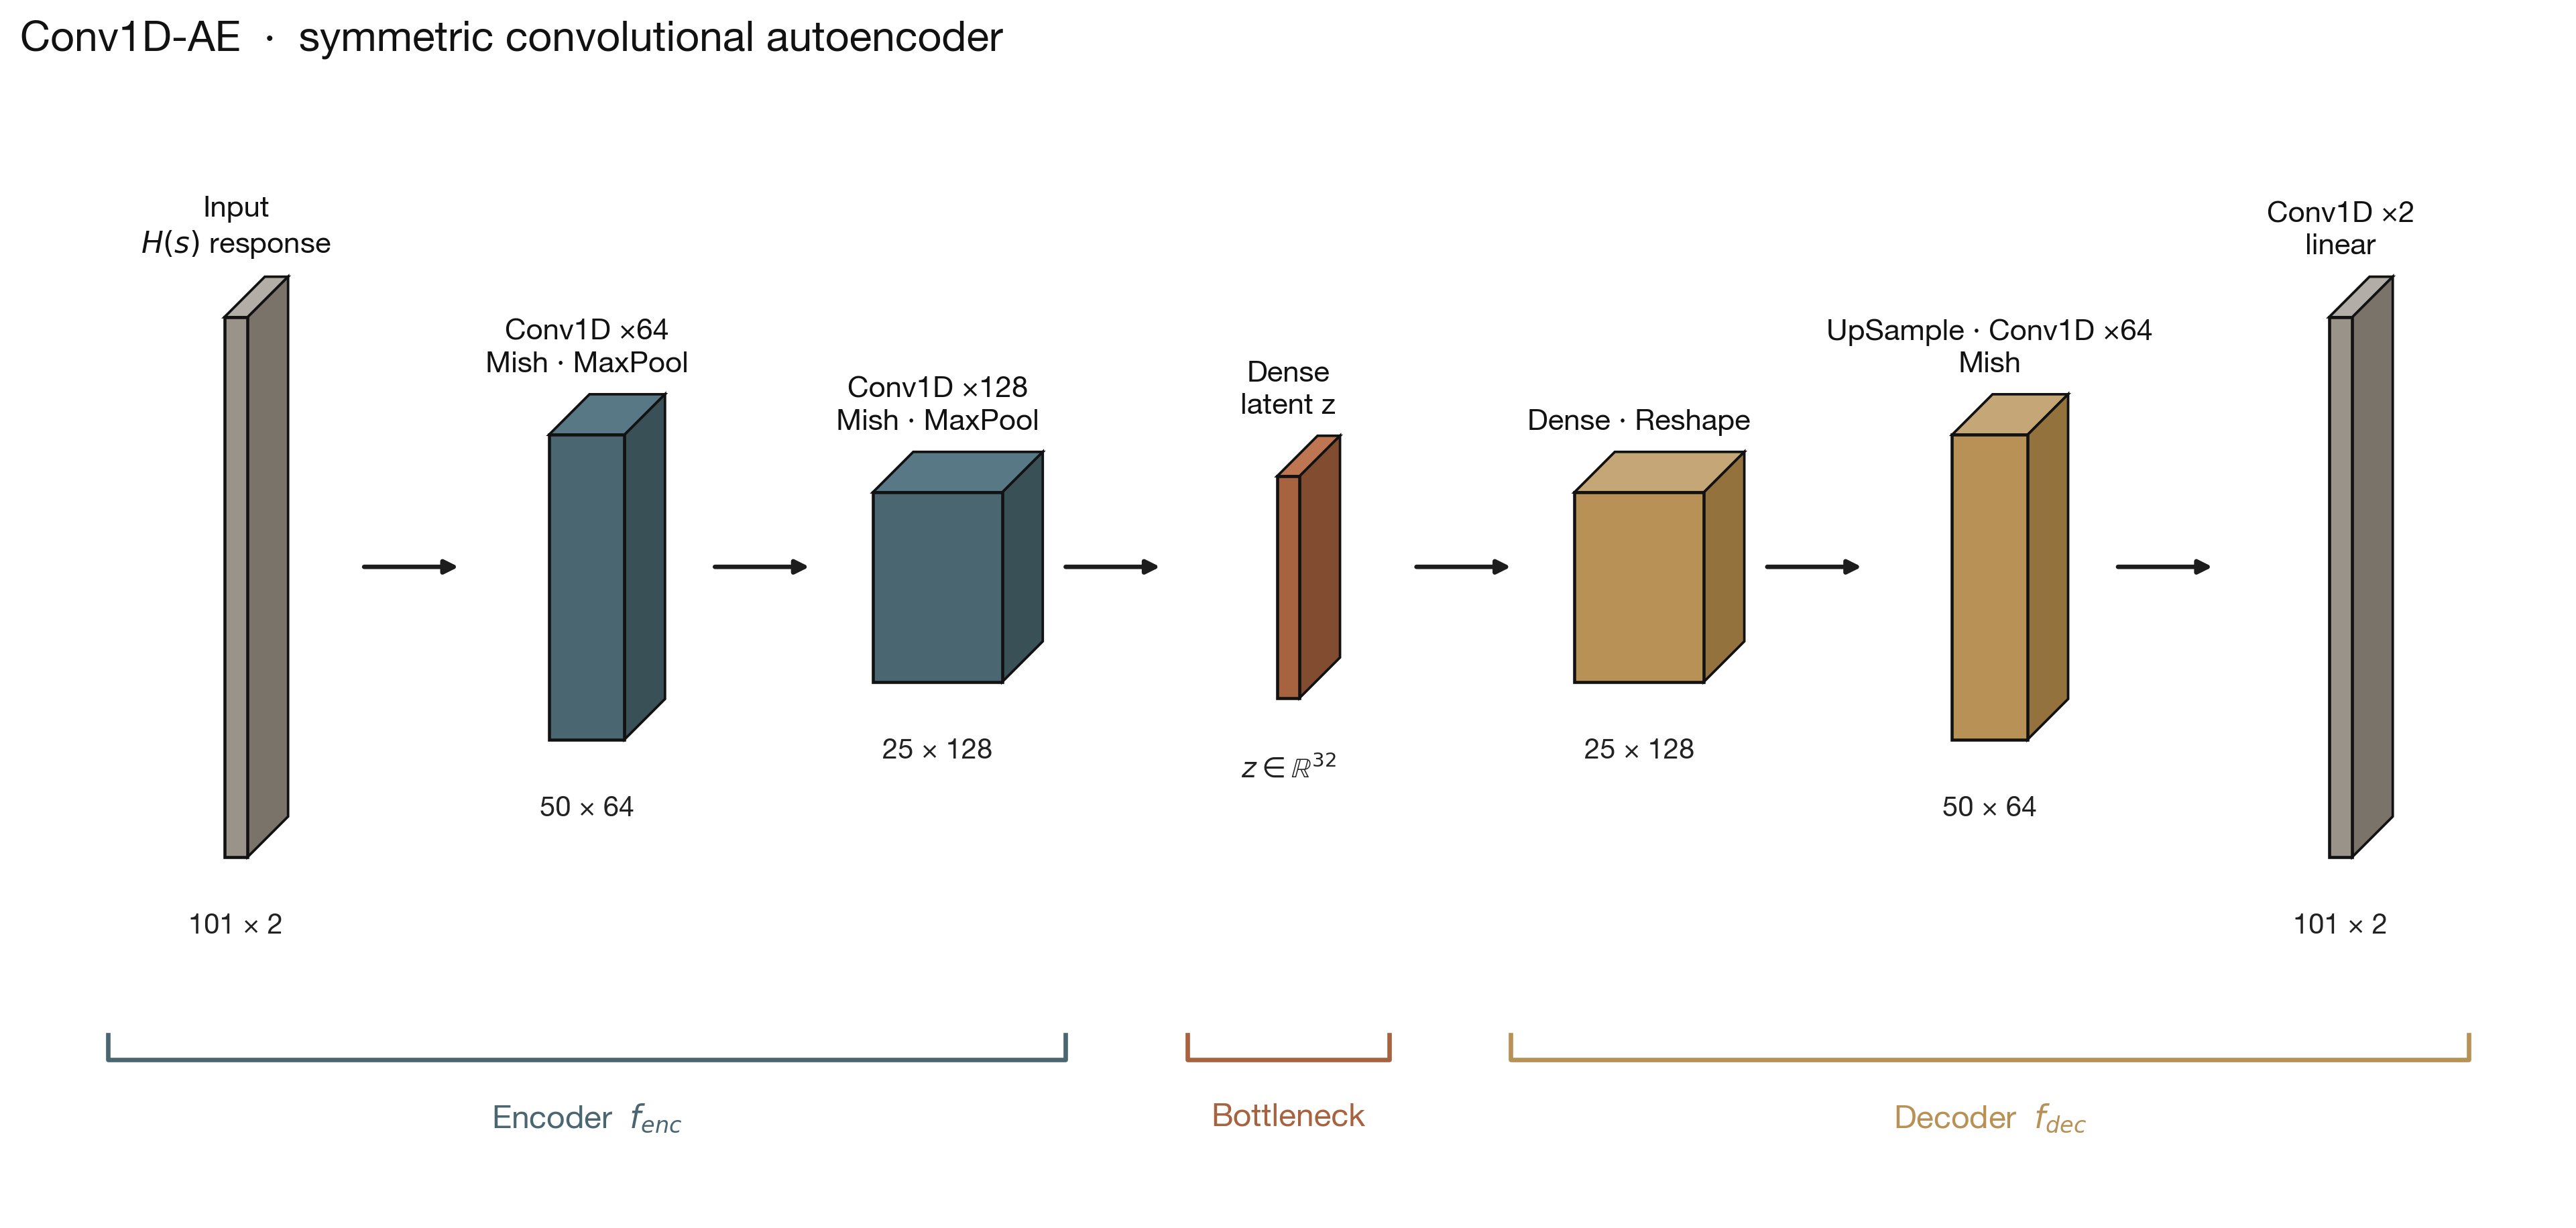
\includegraphics[width=0.9\textwidth]{arch_hero_conv1d_ae.png}
\caption{Conv1D-AE architecture (encoder--bottleneck--decoder), reproduced from the
project's architecture-diagram generator.}
\label{fig:arch-conv1d}
\end{figure}

\section{Physics-Informed Contrastive Anomaly Detection (CARLA)}
\label{sec:carla}

\subsection{Architecture}
CARLA couples an encoder backbone (any of the Conv1D, Transformer, or MLP encoders from
Section~\ref{sec:baselines}) with a projection head (hidden dimension $128$, output
dimension $64$ in the current default configuration) that maps encoder representations
into a space where the contrastive objective is applied (Figure~\ref{fig:arch-carla}). A
reconstruction decoder is retained alongside the projection head so that the training
objective can combine reconstruction and contrastive terms (Section~\ref{sec:objective}).

\begin{figure}[ht]
\centering

\includegraphics[width=0.9\textwidth]{arch_diagram_carla.png}
\caption{CARLA architecture: shared encoder feeding both a reconstruction decoder and a
contrastive projection head.}
\label{fig:arch-carla}
\end{figure}

\subsection{Physics-informed negative synthesis}
\label{sec:physics-negatives}
The central methodological device of this paper is the substitution of CARLA's original,
domain-agnostic negative-sample operators (resonance shifts applied as generic signal
warps, amplitude scaling, phase distortion, spectral noise injection, point drops) with a
\textbf{physics-informed negative sampler}. Given a training signature with (estimated or
known) frequency context, the sampler:
\begin{enumerate}
    \item draws a fault mode from a fixed catalogue of five physically grounded
    perturbations, each defined as a multiplicative range on a component's nominal value:
    capacitor ESR rise ($3$--$8\times$), capacitance drop ($0.3$--$0.7\times$), inductor
    saturation ($0.4$--$0.7\times$), switch (MOSFET) degradation ($3$--$15\times$
    $R_{ds,on}$), and load change ($0.3$--$3\times$, sampled log-uniformly as an
    operating-point rather than a fault);
    \item perturbs the corresponding entry of $\boldsymbol\theta$ and analytically
    re-derives the perturbed transfer function $\tilde H(j\omega)$ via
    Eq.~\eqref{eq:gvd};
    \item forms the negative signature by applying the analytic \emph{ratio} between the
    perturbed and nominal responses to the \emph{observed} nominal signature, i.e.
    $\tilde x(\omega) = x^{(0)}(\omega)\cdot \big|\tilde H(j\omega)\big/H^{(0)}(j\omega)\big|$
    for amplitude (and the corresponding phase shift), rather than perturbing the signal
    with an unconstrained heuristic.
\end{enumerate}
This produces negatives that are, by construction, consistent with a physically
realizable converter state rather than an arbitrary out-of-distribution signal
perturbation. When no frequency context is available for a given batch, the trainer falls
back to the original heuristic injector, so the two negative-sampling strategies can be
compared in a controlled ablation (Section~\ref{sec:setup}).

\subsection{Training objective}
\label{sec:objective}
Positive/negative pairs are optimized with the Normalized Temperature-scaled Cross
Entropy (NT-Xent) loss~\cite{chen2020simclr,darban2023carla}:
\begin{equation}
\mathcal L_{\text{NT-Xent}} = -\log \frac{\exp(\mathrm{sim}(z_i,z_j)/\tau)}{\sum_{k=1}^{2N}\mathbb 1_{[k\neq i]}\exp(\mathrm{sim}(z_i,z_k)/\tau)}\,,
\label{eq:ntxent}
\end{equation}
with temperature $\tau=0.1$, combined with the reconstruction loss into a single training
objective
\begin{equation}
\mathcal L = w_r\,\mathcal L_{\text{recon}} + w_c\,\mathcal L_{\text{NT-Xent}}\,,
\label{eq:combined-loss}
\end{equation}
using the current default weights $w_r=0.1$, $w_c=0.5$.

\subsection{Anomaly scoring}
At inference time, the anomaly score is a non-parametric $k$-nearest-neighbour distance
in the projection space~\cite{cover1967knn},
\begin{equation}
s(x) = \frac{1}{k}\sum_{j\in\mathrm{NN}_k(z_x)} \lVert z_x - z_j \rVert_2\,,
\qquad k=5\,,
\label{eq:knn-score}
\end{equation}
computed against a reference bank of projected healthy training samples. A decision
threshold on $s(x)$ is calibrated by one of several interchangeable rules (percentile of
the healthy-score distribution, mean $+\,n$ standard deviations, F1-optimal search, or
Youden's $J$ statistic~\cite{fawcett2006roc}), and threshold-independent performance is
additionally reported via ROC-AUC and PR-AUC.

\section{Experimental Setup}
\label{sec:setup}

\textbf{Hyperparameter search.} All models are tuned with Bayesian optimization
(Keras Tuner), $30$ trials by default. For CARLA, the search spans encoder type
$\in\{\text{conv1d, lstm, gru, transformer, mlp}\}$, latent dimension
$\in\{16,32,64\}$, and learning rate $\in\{10^{-4}, 5\times10^{-4}, 10^{-3}\}$, optimizing
validation ROC-AUC.

\textbf{Metrics.} Accuracy, precision, recall, F1-score, ROC-AUC, and PR-AUC, computed on
the held-out, stratified test split.

\textbf{Baselines.} The six autoencoder architectures of Section~\ref{sec:baselines},
trained and evaluated under the identical protocol and dataset split as CARLA.

\textbf{Ablation.} To isolate the effect of Section~\ref{sec:physics-negatives}'s
contribution, we train two CARLA variants under otherwise identical configuration:
\textsc{CARLA-Heuristic} (original domain-agnostic negative operators only) and
\textsc{CARLA-Physics} (physics-informed negative sampler). This is the direct empirical
test of whether physically grounded negative synthesis improves discriminative power over
generic signal perturbation.

\textbf{Reproducibility.} See Section~\ref{sec:reproducibility} for the exact commands
used to regenerate every result in Section~\ref{sec:results}.

\section{Results}
\label{sec:results}

\begin{table}[ht]
\centering
\caption{Test-set performance, all architectures. \mocknote}
\label{tab:main-results}
\begin{tabular}{@{}lcccccc@{}}
\toprule
Model & Accuracy & Precision & Recall & F1 & ROC-AUC & PR-AUC \\
\midrule
MLP-AE & [MOCK] & [MOCK] & [MOCK] & [MOCK] & [MOCK] & [MOCK] \\
GRU-AE & [MOCK] & [MOCK] & [MOCK] & [MOCK] & [MOCK] & [MOCK] \\
VAE & [MOCK] & [MOCK] & [MOCK] & [MOCK] & [MOCK] & [MOCK] \\
LSTM-AE & [MOCK] & [MOCK] & [MOCK] & [MOCK] & [MOCK] & [MOCK] \\
Transformer-AE & [MOCK] & [MOCK] & [MOCK] & [MOCK] & [MOCK] & [MOCK] \\
Conv1D-AE & [MOCK] & [MOCK] & [MOCK] & [MOCK] & [MOCK] & [MOCK] \\
\textbf{CARLA-Physics (ours)} & [MOCK] & [MOCK] & [MOCK] & [MOCK] & [MOCK] & [MOCK] \\
\bottomrule
\end{tabular}
\end{table}

\begin{table}[ht]
\centering
\caption{Ablation: physics-informed vs.\ heuristic negative sampling in CARLA. \mocknote}
\label{tab:ablation}
\begin{tabular}{@{}lcccccc@{}}
\toprule
Variant & Accuracy & Precision & Recall & F1 & ROC-AUC & PR-AUC \\
\midrule
CARLA-Heuristic (original operators) & [MOCK] & [MOCK] & [MOCK] & [MOCK] & [MOCK] & [MOCK] \\
CARLA-Physics (this work) & [MOCK] & [MOCK] & [MOCK] & [MOCK] & [MOCK] & [MOCK] \\
$\Delta$ (Physics $-$ Heuristic) & [MOCK] & [MOCK] & [MOCK] & [MOCK] & [MOCK] & [MOCK] \\
\bottomrule
\end{tabular}
\end{table}

\figureplaceholder{roc-curves}{ROC curves for all seven models (six autoencoder baselines
plus CARLA-Physics) on the held-out test set.}

\figureplaceholder{score-separability}{Distribution of the anomaly score $s(x)$
(Eq.~\eqref{eq:knn-score}) for normal vs.\ anomalous test samples, CARLA-Physics vs.\
CARLA-Heuristic, illustrating separability in projection space.}

\figureplaceholder{confusion-matrices}{Confusion matrices for CARLA-Physics and the
strongest autoencoder baseline, broken down by the number of simultaneously faulted
components (single- vs.\ multi-fault samples).}

\section{Discussion}
\label{sec:discussion}

\textit{[Templated --- to be written once Table~\ref{tab:main-results} and
Table~\ref{tab:ablation} contain real numbers; see Section~\ref{sec:reproducibility}.]}
The discussion should address: (i) whether \textsc{CARLA-Physics} improves over
\textsc{CARLA-Heuristic} on the metrics of Table~\ref{tab:ablation}, and whether that
improvement is concentrated on multi-fault samples (Figure~\ref{fig:confusion-matrices})
where generic heuristic negatives are least likely to resemble a real converter state;
(ii) how CARLA-Physics compares to the reconstruction-only baselines of
Table~\ref{tab:main-results}, in particular whether contrastive scoring recovers any
sensitivity gap relative to Conv1D-AE; (iii) any component-wise asymmetry in detection
difficulty (e.g., components whose fault bands are analytically degenerate with another
component's healthy band inside the $100\text{ Hz}$--$50\text{ kHz}$ measurement window,
per the corner-frequency discussion in Section~\ref{sec:problem}).

\section{Conclusion and Future Work}
\label{sec:conclusion}

This paper formalized power-converter frequency-response anomaly detection as a
set-membership labeling problem over standards-grounded component multiplier bands, and
introduced a physics-informed negative sampler for CARLA-style contrastive anomaly
detection that synthesizes negatives by analytically perturbing the converter's own
small-signal model rather than applying domain-agnostic signal heuristics. Pending the
retraining described in Section~\ref{sec:reproducibility}, we expect this physically
grounded negative synthesis to particularly benefit multi-fault detection and sample
efficiency relative to the original heuristic operators. A companion paper submitted to
the \emph{Journal of Supercomputing} addresses the computational optimization and
edge-hardware deployment of the resulting models. Future extensions include
linear-complexity state-space encoders~\cite{gu2023mamba}, embedding the converter's
governing differential equations directly into the contrastive
objective~\cite{raissi2019pinn}, and symbolic-regression-style interpretability via
Kolmogorov--Arnold layers~\cite{liu2024kan}.

\section{Reproducibility}
\label{sec:reproducibility}

Code, the physics-informed negative sampler, and (upon publication) the generated dataset
are available in the project repository. All results in Section~\ref{sec:results} can be
regenerated with:
\begin{verbatim}
PYTHONPATH=. uv run python -m src.train \
  --model carla --n-trials 30 --final-epochs 100 \
  --data-dir data/buck/buck_data \
  --search-method bayesian --objective roc_auc
\end{verbatim}
which trains under the current \texttt{CARLAConfig} default
(\texttt{use\_physics\_anomalies=True}). The heuristic-negative ablation
(\textsc{CARLA-Heuristic}) requires the corresponding configuration flag set to
\texttt{False} (see the project's research plan, \texttt{papers/PLAN.md}, Section~4.1,
for the exact procedure at the time of writing). Baseline autoencoders are trained via
\texttt{scripts/train\_all.sh}.

\section*{Data Availability Statement}
The simulated dataset and generation code will be made publicly available upon
publication, consistent with the project's stated open-source intent.

\section*{Conflict of Interest Statement}
\textit{[TODO --- to be completed by the authors; assumed ``The authors declare no
conflict of interest'' pending confirmation.]}

\section*{Acknowledgements}
\textit{[TODO --- funding sources and institutional acknowledgements to be added by the
authors.]}

\bibliographystyle{unsrt}
\bibliography{../shared/references}

\end{document}
